\section{Quantencomputer}
\subsection{Entwicklung} 
Die Grundidee der Quantencomputer findet ihren Ursprung im Jahr 1980, 
als Paul Benioff ein theoretisches Modell einer klassischen Turing-Maschine beschrieb, 
die den Gesetzen der Quantenmechanik unterlag.
Benioff demonstrierte, dass die Zustände einer Turing-Maschine in einem Quantensystem darstellbar sind. 
Er zeigte außerdem, dass klassische Operationen, die in einer Turing-Maschine ausgeführt werden, 
durch entsprechende Quantengatter auf einem Quantensystem äquivalent durchgeführt werden können~\cite{benioff1980}.

Kurz nach der Veröffentlichung von Benioffs Arbeit beschäftigte sich Richard Feynman im Jahr 1981 mit der Frage,
wie effizient ein klassischer Computer bei der Simulation physikalischer Prozesse ist.
Feynman befasste sich mit der Schwierigkeit, die Quantenmechanik mithilfe eines klassischen Computers zu simulieren.
Er stellte fest, dass die Anforderungen für die Simulation der Quantenmechanik auf einem klassischen Computer mit jedem zusätzlichen Quantenteilchen exponentiell ansteigen.
Die Begründung dafür liegt in der exponentiell wachsenden Menge an Zustandsinformationen,
die für die Beschreibung des Quantensystems benötigt werden.
Als Lösungsansatz nannte Feynman einen Quantencomputer, 
der selbst auf den Prinzipien der Quantenmechanik basiert und dadurch eine effiziente Simulation von Quantensystemen ermöglicht~\cite{Feynman1982}.

David Deutsch präsentierte im Jahr 1985 den ersten Quantenalgorithmus, 
der eine spezifische Fragestellung effizienter lösen konnte als alle bekannten klassischen Algorithmen. 
Allerdings bezog sich die betrachtete Fragestellung auf ein Problem von eher theoretischer Natur, 
in dem es darum ging, 
zu ermitteln, ob eine Funktion mit lediglich zwei möglichen Eingaben konstant oder balanciert ist.
Ein klassischer Algorithmus würde zur Beantwortung dieser Frage zwei Funktionsauswertungen benötigen. 
Der Quantenalgorithmus benötigt hingegen
nur eine einzige Funktionsauswertung~\cite{deutsch1985}.

Im Jahr 1994 stellte Shor einen Quantenalgorithmus vor, der in der Lage ist, 
die Ordnung beziehungsweise Periode eines Elements in einer multiplikativen Gruppe eines Modulus mit nur polynomialem Aufwand zu ermitteln. 
Da trotz erheblicher Anstrengungen lediglich klassische Algorithmen mit exponentiellem Aufwand für diese Berechnung zur Verfügung stehen, 
stellte Shors Entdeckung eine Errungenschaft dar, die das allgemeine Interesse für Quantencomputing enorm anregte~\cite{Shor_1997}.

Zwei Jahre später stellte Lov K. Grover einen Quantenalgorithmus vor.
Genau wie der Quantenalgorithmus von Shor kann auch Grovers Quantenalgorithmus ein bestimmtes Problem effizienter lösen als jeglicher klassischer Algorithmus.
Dieser Quantenalgorithmus ermöglicht die Suche in einer unsortierten Datenbank mit einem Aufwand von \(\Landau(\sqrt N)\), 
während der beste klassische Suchalgorithmus diese Aufgabe in \(\Landau(N)\) bewältigt. 
Darüber hinaus zeigte Grover, 
dass es selbst unter vollständiger Ausnutzung der Prinzipien der Quantenmechanik nicht möglich ist, 
die unstrukturierte Suche in weniger als \(\Landau(\sqrt N)\) Schritten durchzuführen~\cite{grover1996fast}.

Die erste erfolgreiche physikalische Implementation eines Quantenalgorithmus wurde im Jahr 1998 durchgeführt.
In dem Versuch wurde der Quantenalgorithmus von David Deutsch auf einem Zwei-Qubit-Quantencomputer implementiert.
Der verwendete Quantencomputer nutzte die Technologie der Kernspinresonanz, 
wobei die zwei Qubits durch Ausnutzung der Spin-Zustände von Atomkernen in spezifischen Molekülstrukturen realisiert wurden~\cite{Jones_1998}.

In der fortlaufenden Entwicklung der Quanteninformationstechnologie wurden verschiedene Arten von Quantencomputern konzeptioniert und realisiert.
Zu diesen zählen adiabatische Quantencomputer, Schaltkreis-basierte und topologische Quantencomputer.
Im Kontext des Quantencomputing wird der Begriff "`Quantencomputer"' oft auf universell einsetzbare Quantencomputer angewendet.
Die Eigenschaft "`universell"' wird in dem Zusammenhang gemäß DiVincenzos Kriterien definiert. 
Im Wesentlichen besagen DiVincenzos Kriterien, dass ein universeller Quantencomputer in der Lage sein muss, jede Quantenberechnung auszuführen, vorausgesetzt, er verfügt über ausreichende Ressourcen~\cite{DiVincenzo_2000}.
Schaltkreis-basierte und topologische Quantencomputer erfüllen DiVincenzos Kriterien und gelten somit als universelle Quantencomputer.
Hingegen sind adiabatische Quantencomputer nicht universell programmierbar und werden explizit zum Lösen von Optimierungsproblemen eingesetzt.

Das Unternehmen International Business Machines (IBM) präsentierte im Jahr 2019 den ersten kommerziell verfügbaren, Schaltkreis-basierten Quantencomputer.
Dieses System, bekannt als "`IBM Q System One"', verfügt über 20 Qubits.
Seit der Vorstellung des System One hat IBM die Qubit-Kapazität kontinuierlich erhöht. 
Aktuelle Systeme, wie die in der Abbildung~\ref{fig:IBM-Quantum-DevRoadmap2022} dargestellt sind, verfügen über bis zu 433 Qubits.
\begin{figure} [H]
\caption{IBM-Quantum-Roadmap~\cite{IBM_2023}}
\label{fig:IBM-Quantum-DevRoadmap2022}
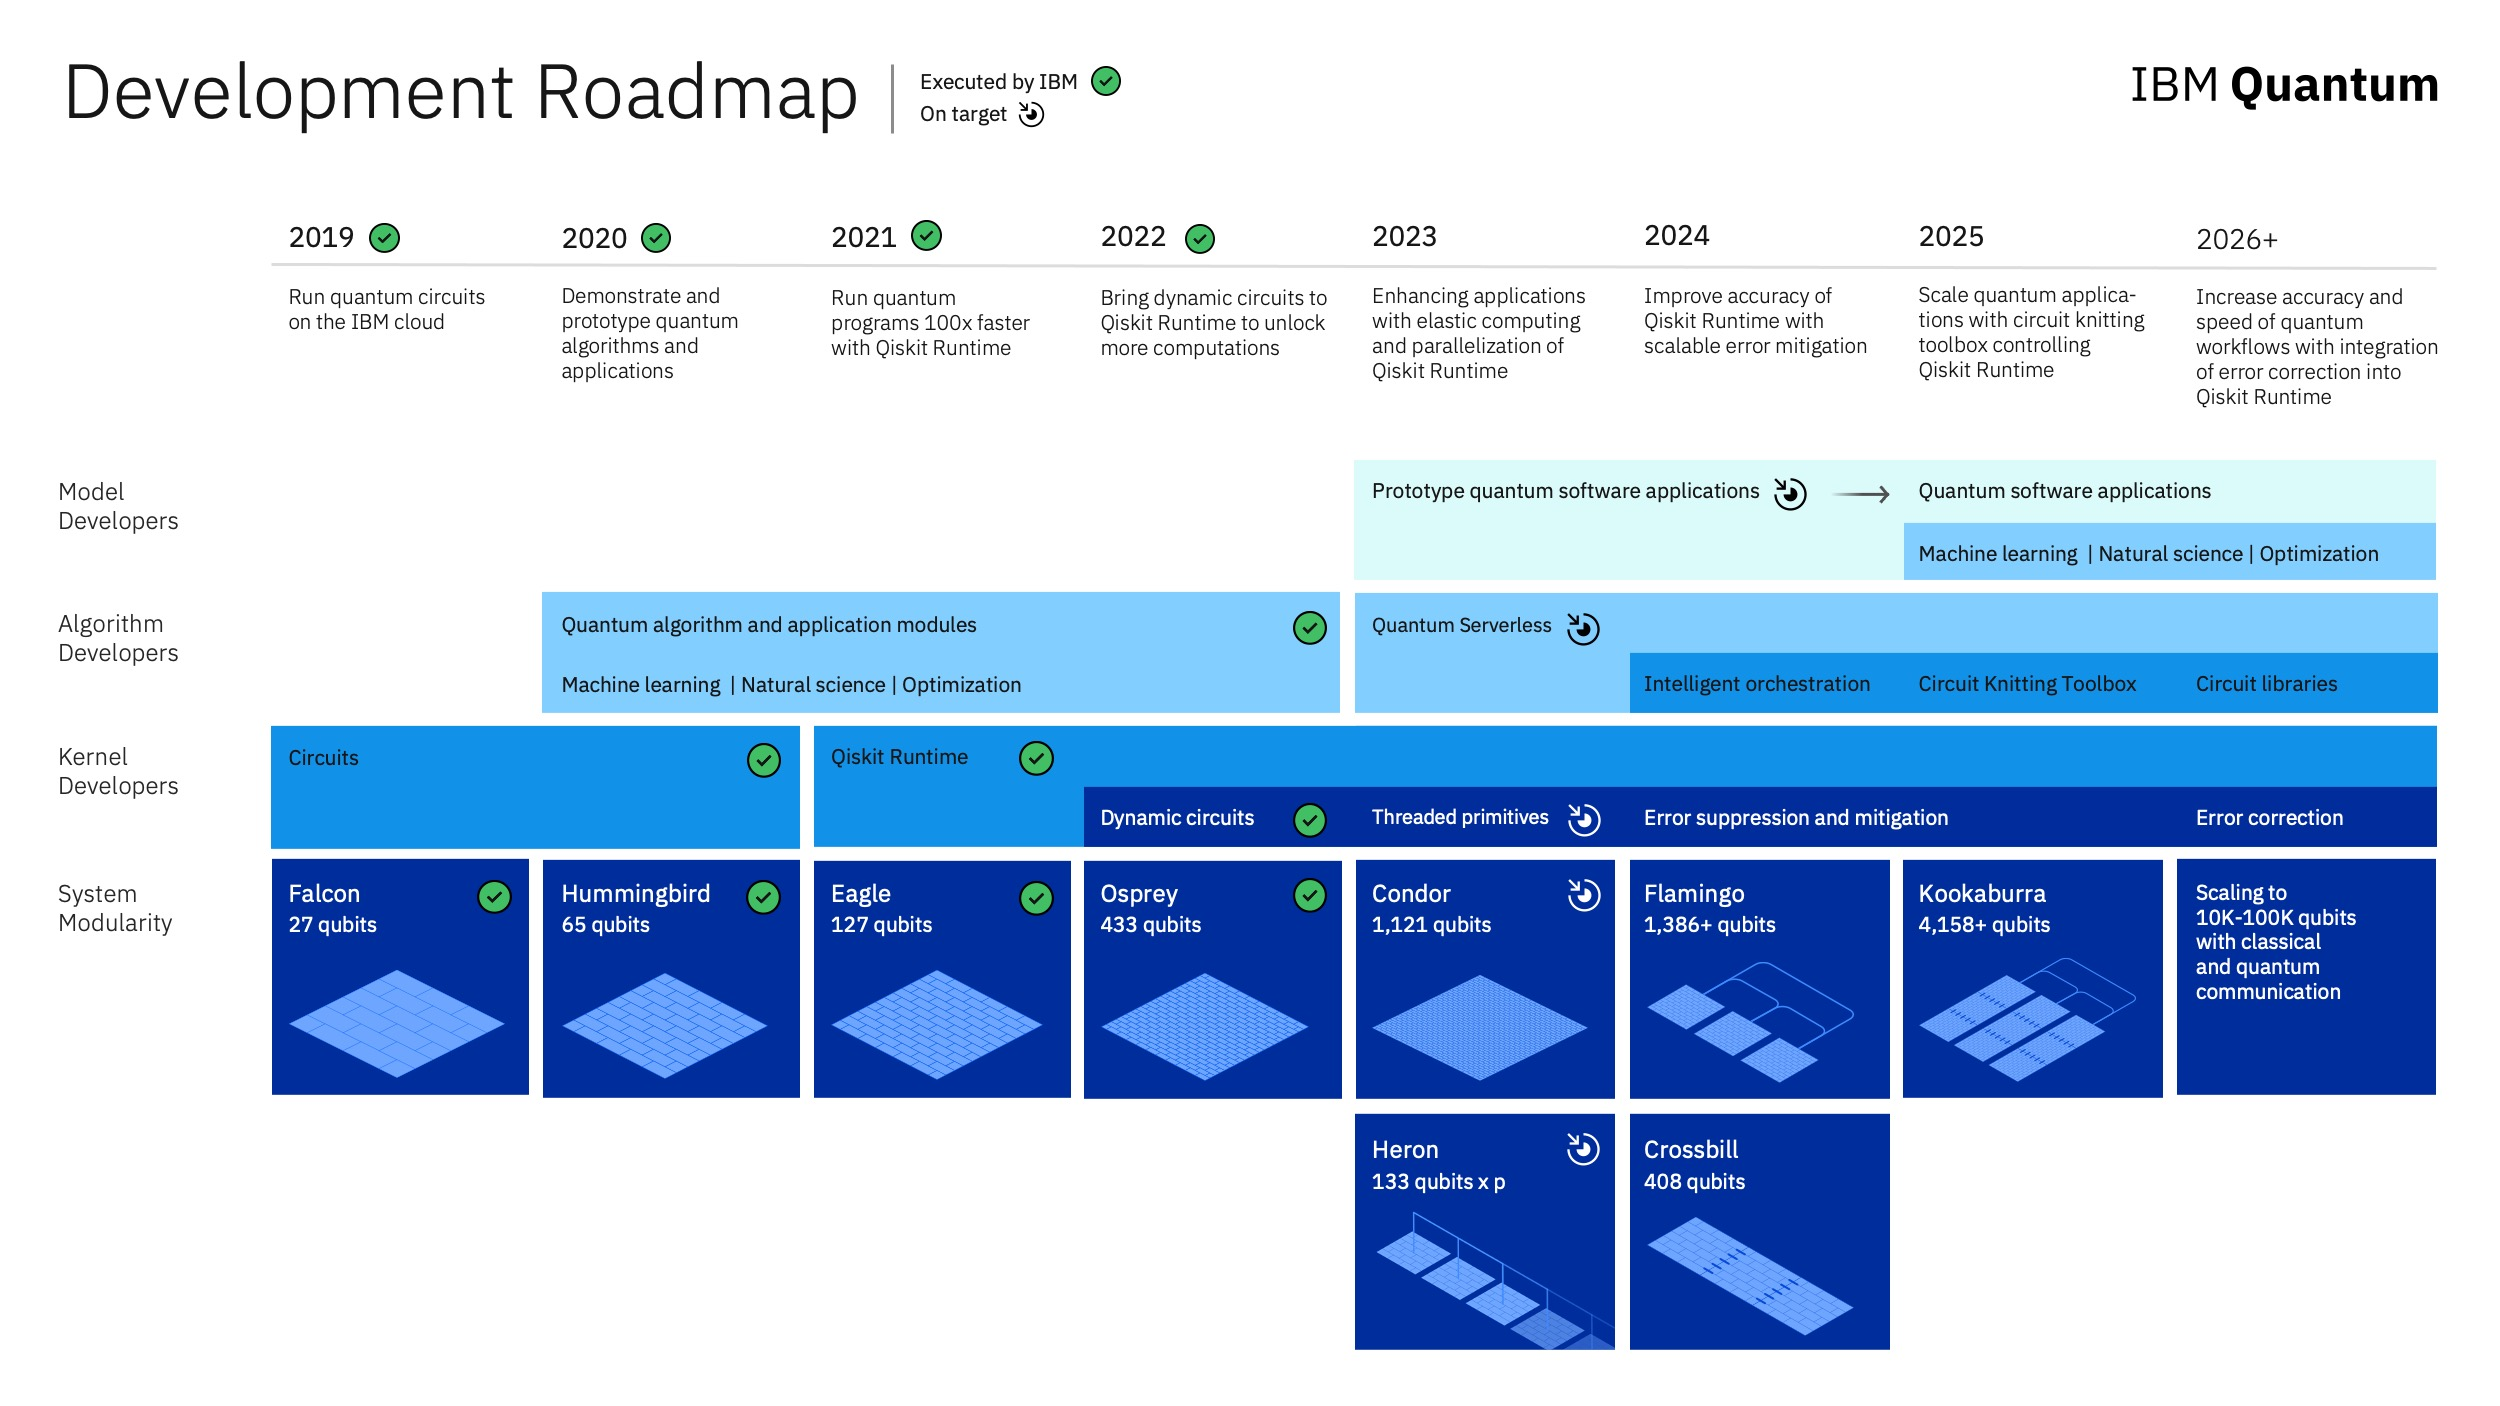
\includegraphics[width=\columnwidth]{IBM-Quantum-DevRoadmap2022_Light.jpeg}
\centering
\end{figure}

In Anbetracht zukünftiger Entwicklungen haben Unternehmen wie Google, IBM und Microsoft umfangreiche Pläne zur Erweiterung ihrer Quantencomputing-Kapazitäten. 
Google plant beispielsweise die Errichtung eines Quanten-Campus, der bis 2030 über einen Quantencomputer mit einer Million Qubits verfügen soll~\cite{Google_2023}. 
Microsoft verfolgt ähnliche Ziele, wobei der konkrete Umfang ihrer Projekte bislang nicht öffentlich spezifiziert wurde.
Des Weiteren erwartet das Bundesamt für Sicherheit in der Informationstechnik die Existenz kryptografisch relevanter Quantencomputer zu Beginn der 2030er Jahre~\cite{BSI_KPMG_2023}. 

\subsection{Vorteile gegenüber klassischen Rechnern} 
Quantenparallelismus 
